
\addchap{Essay: Software engineers and software artisans}

Let us examine what we ordinarily understand by \emph{engineering}
as opposed to artisanship or craftsmanship. It will then become apparent
that today\textsf{'}s computer programmers must be viewed as \textsf{``}software artisans\textsf{''}
rather than software engineers.

\addsec{Engineering disciplines }

Consider the way mechanical engineers, chemical engineers, or electrical
engineers work, and look at the studies they require for becoming
proficient in their fields.

A mechanical engineer studies calculus, linear algebra, differential
geometry, and several areas of physics such as theoretical mechanics,
thermodynamics, and elasticity theory,\footnote{\texttt{\href{https://www.colorado.edu/mechanical/academics/undergraduate-program/curriculum}{https://www.colorado.edu/mechanical/academics/undergraduate-program/curriculum}}}
and then uses calculations to guide the design of a bridge. A chemical
engineer studies chemistry, thermodynamics, calculus, linear algebra,
differential equations, some areas of physics such as thermodynamics
and kinetic theory,\footnote{\texttt{\href{https://www.colorado.edu/engineering/sample-undergraduate-curriculum-chemical}{https://www.colorado.edu/engineering/sample-undergraduate-curriculum-chemical}}}
and uses calculations to guide the design of a chemical process. An
electrical engineer studies advanced calculus, linear algebra, and
several areas of physics such as electrodynamics and quantum theory,\footnote{\texttt{\href{http://archive.is/XYLyE}{http://archive.is/XYLyE}}}
and uses calculations to design an antenna or a microchip.

The common pattern is that engineers use mathematics and natural sciences
in order to create new devices. Mathematical calculations and scientific
reasoning are performed \emph{before} designing or building a real
machine.

Some of the studies required for engineers include arcane abstract
concepts such as the \textsf{``}Fourier transform of the delta function\textsf{''}\footnote{\texttt{\href{https://www.youtube.com/watch?v=KAbqISZ6SHQ}{https://www.youtube.com/watch?v=KAbqISZ6SHQ}}}
and the \textsf{``}inverse $Z$-transform\textsf{''}\footnote{\texttt{\href{http://archive.is/SsJqP}{http://archive.is/SsJqP}}}
in digital signal processing, \textsf{``}rank 4 tensors\textsf{''}\footnote{\texttt{\href{https://serc.carleton.edu/NAGTWorkshops/mineralogy/mineral_physics/tensors.html}{https://serc.carleton.edu/NAGTWorkshops/mineralogy/mineral\_physics/tensors.html}}}
in calculations of elasticity of materials, \textsf{``}Lagrangians with non-holonomic
constraints\textsf{''}\footnote{\texttt{\href{https://arxiv.org/abs/math/0008147}{https://arxiv.org/abs/math/0008147}}}
in robotics, and the \textsf{``}Gibbs free energy\textsf{''} in chemical reactor design.\footnote{\texttt{\href{https://amzn.com/dp/1118368258}{https://amzn.com/dp/1118368258}}}

To be sure, a significant part of what engineers do is not covered
by any theory: the \emph{know-how}, the informal reasoning, the traditional
knowledge passed on from expert to novice,  \textemdash{} all those
skills that are hard to formalize are important. Nevertheless, engineering
is crucially based on natural science and mathematics for some of
its decision-making about new designs.

\addsec{Artisanship: Trades and crafts }

Now consider what kinds of things shoemakers, plumbers, or home painters
do, and what they have to learn in order to become proficient in their
profession.

A novice shoemaker, for example, begins by copying some drawings\footnote{\texttt{\href{https://youtu.be/cY5MY0czMAk?t=141}{https://youtu.be/cY5MY0czMAk?t=141}}}
and goes on to cutting leather in a home workshop. Apprenticeships
proceed via learning by doing, with comments and instruction from
an expert. After a few years of study (for example, a painter apprenticeship
in California can be as short as two years\footnote{\texttt{\href{http://www.calapprenticeship.org/programs/painter_apprenticeship.php}{http://www.calapprenticeship.org/programs/painter\_apprenticeship.php}}}),
a new artisan is ready to start productive work. 

All trades operate entirely from tradition and practical experience.
It takes a prolonged learning effort to become a good artisan in any
profession. But the trades do not require academic study because there
is no formal theory from which to proceed. There are no Fourier transforms
applied to delta functions, no Lagrangians with non-holonomic constraints,
no fourth rank tensors to calculate, nor any differential equations
to solve.

Artisans do not study science or mathematics because their professions
do not make use of any formal theory for guiding their designs or
processes.

\addsec{Programmers today are artisans, not engineers }

Programmers are \emph{not engineers} in the sense normally used in
the engineering professions.

\subsection*{No requirements of licensing or formal study}

Mechanical, electrical, chemical engineers are required to pass a
license exam to become certified to work. The license exam certifies
that the person is proficient in applying a known set of engineering
tools and methods. But in software engineering, no certifications
or licenses are required for the job (although many certification
programs exist).

Working software engineers are also not required to have studied software
engineering or computer science (CS). According to a recent Stack
Overflow survey,\footnote{\texttt{\href{https://thenextweb.com/insider/2016/04/23/dont-need-go-college-anymore-programmer/}{https://thenextweb.com/insider/2016/04/23/dont-need-go-college-anymore-programmer/}}}
about 56\% of working programmers have no CS degree. The author of
this book is a self-taught programmer who has degrees in physics but
never formally studied CS or taken any academic courses in algorithms,
data structures, computer networks, compilers, programming languages,
or other standard CS topics. 

A large fraction of successful programmers have no college degrees
and perhaps \emph{never} studied formally. They acquired all their
knowledge and skills through self-study and practical work. A prominent
example is Robert C.~Martin\index{Robert C.~Martin},\footnote{\texttt{\href{https://en.wikipedia.org/wiki/Robert_C._Martin}{https://en.wikipedia.org/wiki/Robert\_C.\_Martin}}}
an outspoken guru in the arts of programming. He routinely refers
to programmers as artisans\footnote{\texttt{\href{https://blog.cleancoder.com/uncle-bob/2013/02/01/The-Humble-Craftsman.html}{https://blog.cleancoder.com/uncle-bob/2013/02/01/The-Humble-Craftsman.html}}}
and uses the appropriate imagery: novices and masters, trade and craft,
the honor of the guild, etc. He compares programmers to plumbers,
electricians, lawyers, and surgeons, but never to mathematicians,
physicists, or engineers of any kind. According to one of his blog
posts,\footnote{\texttt{\href{https://blog.cleancoder.com/uncle-bob/2013/11/25/Novices-Coda.html}{https://blog.cleancoder.com/uncle-bob/2013/11/25/Novices-Coda.html}}}
he started working at age 17 as a self-taught programmer. He never
went to college and holds no degrees.\footnote{\texttt{\href{https://hashnode.com/post/i-am-robert-c-martin-uncle-bob-ask-me-anything-cjr7pnh8g000k2cs18o5nhulp/2}{https://archive.is/MNlgT}}}
It is clear that R.~C.~Martin \emph{is} an expert craftsman and
that he did \emph{not} need academic study to master the craft of
programming.

Here is another opinion\footnote{\texttt{\href{http://archive.is/tAKQ3}{http://archive.is/tAKQ3}}}
(emphasis is theirs):
\begin{quotation}
{\small{}Software Engineering is unique among the STEM careers in
that it absolutely does }\emph{\small{}not}{\small{} require a college
degree to be successful. It most certainly does not require licensing
or certification. }\emph{\small{}It requires experience}{\small{}.}{\small\par}
\end{quotation}
This description fits a career in crafts \textemdash{} but certainly
not a career, say, in electrical engineering.

The high demand for software developers gave rise to \textsf{``}developer
boot camps\textsf{''}\footnote{\texttt{\href{http://archive.is/GkOL9}{http://archive.is/GkOL9}}}
\textemdash{} vocational schools that educate new programmers in a
few months through purely practical training, with no formal theory
or mathematics involved. These vocational schools are successful\footnote{\texttt{\href{http://archive.is/E9FXP}{http://archive.is/E9FXP}}}
in job placement. But it is unimaginable that a $6$-month crash course
or even a $2$-year vocational school could prepare engineers to work
successfully on designing, say, analog quantum computers\footnote{\texttt{\href{https://www.dwavesys.com/quantum-computing}{https://www.dwavesys.com/quantum-computing}}}
without ever learning quantum physics or calculus.

\subsection*{No mathematical formalism guides software development}

Most books on software engineering contain no formulas or equations,
no mathematical derivations, and no precise definitions of the various
technical terms they are using (such as \textsf{``}object-oriented\textsf{''} or \textsf{``}module\textsf{'}s
responsibilities\textsf{''}). Some of those books\footnote{E.g., \texttt{\href{https://amzn.com/dp/0073376256}{https://amzn.com/dp/0073376256}}}
also have almost no program code in them. Some of those books are
written by practitioners such as R.\ C.\ Martin who do not explain
their material in terms of formalisms. Instead, they summarize their
programming experience in heuristically formulated \textquotedblleft principles\textquotedblright .\footnote{\texttt{\href{https://blog.cleancoder.com/uncle-bob/2016/03/19/GivingUpOnTDD.html}{https://blog.cleancoder.com/uncle-bob/2016/03/19/GivingUpOnTDD.html}}}
The programmers are told: \textsf{``}code is about detail\textsf{''}, \textsf{``}never abandon
the big picture\textsf{''}, \textsf{``}avoid tight coupling in your modules\textsf{''}, \textsf{``}a
class must serve a single responsibility\textsf{''}, \textsf{``}strive for good interfaces\textsf{''},
and so on. 

In contrast, textbooks on mechanical or electrical engineering include
a significant amount of mathematics. The design of a microwave antenna
is guided not by an \textsf{``}open and closed module principle\textsf{''} but by
solving the relevant differential equations\footnote{\texttt{\href{https://youtu.be/8KpfVsJ5Jw4?t=447}{https://youtu.be/8KpfVsJ5Jw4?t=447}}}
of electrodynamics.

Another example of programmers\textsf{'} avoidance of mathematical tools is
given by the \textsf{``}Liskov substitution principle\index{Liskov substitution principle}\textsf{''}
for subtyping\index{subtyping}.\footnote{See \texttt{\href{https://en.wikipedia.org/wiki/Liskov_substitution_principle}{https://en.wikipedia.org/wiki/Liskov\_substitution\_principle}}.
The LSP always holds in functional programming if values are immutable
and subtyping is viewed as an automatic type conversion function (see
Definition~\ref{subsec:Definition-subtyping}). A property $\phi(y)$
is rewritten as $\phi(c(y))$ by inserting a suitable type conversion
function, $c:S\rightarrow T$. Since $c(y)$ has type $T$ and $\phi(x)$
holds for all values $x:T$,  the property $\phi(c(y))$ holds automatically.} Its rigorous formulation (\textsf{``}for any property $\phi(x)$ that holds
for all $x$ of type $T$, and for any subtype $S$ of $T$, the property
$\phi(y)$ must also hold for all $y$ of type $S$\textsf{''}) is not used
by programmers. Instead, the literature on object-oriented programming
formulates the principle as \textsf{``}objects of type $T$ may be substituted
by objects of type $S$ while keeping the correctness of the program\textsf{''}.
This formulation \index{object-oriented programming} is both vague
(it does not specify how to choose the substituted objects of type
$S$) and, strictly speaking, incorrect: If the program contains a
function $f(t)$ where $t$ is a value of type $T$, it is not always
possible to find some value $s$ of type $S$ such that $f(s)=f(t)$.
The reason is that some subtyping relations are not surjective, as
shown in Section~\ref{subsec:Subtyping-with-injective} of this book.

Donald Knuth\textsf{'}s classic textbook \textsf{``}\emph{The Art of Programming}\textsf{''}
indeed treats programming as an art and not as a science. Knuth shows
many algorithms and derives their mathematical properties but does
not provide any theory that could guide programmers in actually \emph{writing}
programs (say, choosing the data types to be used). Knuth assumes
that the reader who understands the mathematical properties of an
algorithm will be able \emph{somehow} to write correct code.

The books \textsf{``}The Science of Programming\textsf{''}\footnote{\texttt{\href{https://amzn.com/dp/0387964800}{https://amzn.com/dp/0387964800}}}
and \textsf{``}Program derivation\textsf{''}\footnote{\texttt{\href{https://amzn.com/dp/0201416247}{https://amzn.com/dp/0201416247}}}
are attempts to provide a mathematical basis for writing programs
starting from formal specifications. The books give some methods that
guide programmers in writing code and at the same time produce a proof
that the code conforms to the specification. However, the scope of
proposed methods is limited to designing algorithms for iterative
manipulation of data, such as sorting and searching algorithms. The
procedures suggested in those books are far from a formal mathematical
\emph{derivation} of a wide range of software programs from specifications.
In any case, most programmers today are unaware of these books and
do not use the methods explained there, even when those methods could
apply.

Today\textsf{'}s computer science courses do not teach a true engineering approach
to software construction. Some courses teach analysis of programs
using mathematical methods. Two such methods are complexity analysis\footnote{\texttt{\href{https://www.cs.cmu.edu/~adamchik/15-121/lectures/Algorithmic\%20Complexity/complexity.html}{https://archive.is/6D796}}}
(the \textsf{``}big-$O$ notation\textsf{''}) and formal verification.\footnote{\texttt{\href{https://en.wikipedia.org/wiki/Formal_verification}{https://en.wikipedia.org/wiki/Formal\_verification}}}
But programs are analyzed or verified only \emph{after} they are somehow
written. Theory does not guide the actual \emph{process} of writing
code: it does not define good ways of organizing the code (e.g., how
to decompose the code into modules, classes, or functions) and does
not tell programmers which data structures and type signatures of
functions will be useful to implement. Programmers make these design
decisions on the basis of experience and intuition, trial-and-error,
copy-paste, guesswork, and debugging. 

In a sense, program analysis and verification is analogous to writing
mathematical equations for the surface of a shoe made by a fashion
designer. The resulting \textsf{``}shoe equations\textsf{''} are mathematically rigorous
and could be analyzed or verified. But the equations are merely written
after the fact, they do not guide the fashion designers in actually
making shoes. It is understandable that fashion designers do not study
the mathematical theory of geometric surfaces.

\subsection*{Programmers avoid academic terminology }

Programmers jokingly grumble about terms such as \textsf{``}functor\textsf{''} and
\textsf{``}monad\textsf{''}:
\begin{quote}
{\small{}Those fancy words used by functional programmers purists
really annoy me. Monads, functors... Nonsense!!! }\footnote{\texttt{\href{http://archive.is/65K3D}{http://archive.is/65K3D}}}
\end{quote}
Perhaps only a small minority of software developers complain about
this, as the majority seems to be unaware of \textsf{``}applicative functors\textsf{''},
\textsf{``}free monads\textsf{''}, and other arcane terminology. Indeed, that sort
of terminology is intentionally avoided by most books and tutorials
aimed at programmers.\footnote{For example, the recent book \textsf{``}Grokking functional programming\textsf{''}
\emph{never} mentions \textsf{``}functors\textsf{''} or \textsf{``}monads\textsf{''}. See \texttt{\href{https://www.manning.com/books/grokking-functional-programming}{https://www.manning.com/books/grokking-functional-programming}}}

But why would an \emph{engineer} wince at \textsf{``}functors\textsf{''} or at \textsf{``}free
monads\textsf{''}? Other branches of engineering use lots of terminology that
is far from self-explanatory and requires some study. Chemical engineers
learn about \textsf{``}Gibbs free energy\textsf{''}, which is a technical term that
denotes a certain function. (It\index{jokes} does not mean getting
energy from J.~W.~Gibbs\index{Josiah Willard Gibbs} for free!)
Chemical engineers accept the need for studying \textsf{``}phase diagrams\textsf{''}
and \textsf{``}Fourier\textsf{'}s law\textsf{''}. Mechanical engineers take it for granted
that they have to work with \textsf{``}rank 4 tensors\textsf{''}, \textsf{``}Lagrangians\textsf{''},
and \textsf{``}non-holonomic constraints\textsf{''}. Electrical engineers do not avoid
\textsf{``}Fourier transforms\textsf{''} or \textsf{``}delta functions\textsf{''} just because those
are weird things to say. The arcane terminology seems to be the least
of their difficulties, as their textbooks are full of complicated
equations and long derivations.

Textbooks on true software engineering would have been full of equations
and derivations, teaching engineers how to perform certain calculations
that are required \emph{before} starting to write code.

\addsec{Towards true engineering in software}

It is now clear that we do not presently have true software engineering.
The people employed under that job title are actually artisans. They
work using artisanal methods, and their education and design processes
are typical of a crafts guild.

Software engineering in the proper sense would mean having a mathematical
theory that guides the process of writing programs, \textemdash{}
not just theory that describes or analyzes programs after they are
\emph{somehow} written.

It is true that numerical methods required for physics and matrix
calculations required for data science are \textsf{``}mathematical\textsf{''}. Those
programming tasks are indeed formulated using mathematical theory.
However, mathematical \emph{subject matter} (aerospace control, physics
simulations, or statistics) corresponds to a relatively small part
of written code and does not by itself guide the process of writing
code. Data scientists, aerospace engineers, and physicists almost
always work as artisans when converting their computations into program
code.

We expect that software engineers\textsf{'} textbooks should be full
of equations and derivations. What theory would those equations represent?

This theory is what this book calls \textbf{applied functional type
theory}\index{applied functional type theory} (see Chapter~\ref{chap:Applied-functional-type}).
It represents the mathematical foundation of the modern practice of
functional programming, as implemented in languages such as OCaml,
Haskell, and Scala. This theory is a blend of set theory, category
theory, and logical proof theory, adapted for the needs of programmers.
It has been in development since late 1990s and is still being actively
worked on by a community of software practitioners and academic computer
scientists.

To appreciate that functional programming, unlike other paradigms,
is based on a \emph{theory that guides coding}, we can look at some
recent software engineering conferences such as \textsf{``}Scala By the Bay\textsf{''}\footnote{\texttt{\href{http://2015.scala.bythebay.io/}{http://2015.scala.bythebay.io/}}}
or BayHac,\footnote{\texttt{\href{http://bayhac.org/}{http://bayhac.org/}}}
or at the numerous FP-related online tutorials and blogs. We cannot
fail to notice that speakers devote significant time to a peculiar
kind of applied mathematical reasoning. Rather than focusing on one
or another API or algorithm, as it is often the case with other software
engineering blogs or presentations, an FP speaker describes a \emph{mathematical
structure} \textemdash{} such as the \textsf{``}applicative functor\textsf{''}\footnote{\texttt{\href{http://www.youtube.com/watch?v=bmIxIslimVY}{http://www.youtube.com/watch?v=bmIxIslimVY}}}
or the \textsf{``}free monad\textsf{''}\footnote{\texttt{\href{http://www.youtube.com/watch?v=U0lK0hnbc4U}{http://www.youtube.com/watch?v=U0lK0hnbc4U}}}
\textemdash{} and illustrates its use for practical coding.

These people are not graduate students showing off their theoretical
research. They are practitioners, software engineers who use FP on
their jobs. It is just the nature of FP that certain mathematical
tools and constructions are directly applicable to practical programming
tasks.

These mathematical tools are not mere tricks for a specific programming
language; they apply equally to all FP languages. Before starting
to write code, the programmer can jot down certain calculations in
a mathematical notation (see Fig.\ \ref{fig:Example-calculation-in-type-theory}).
The results of those calculations will help design the code fragment
the programmer is about to write. This activity is similar to that
of an engineer who performs some mathematical calculations before
embarking on a design project. 

\begin{figure}
\begin{centering}
{\footnotesize{}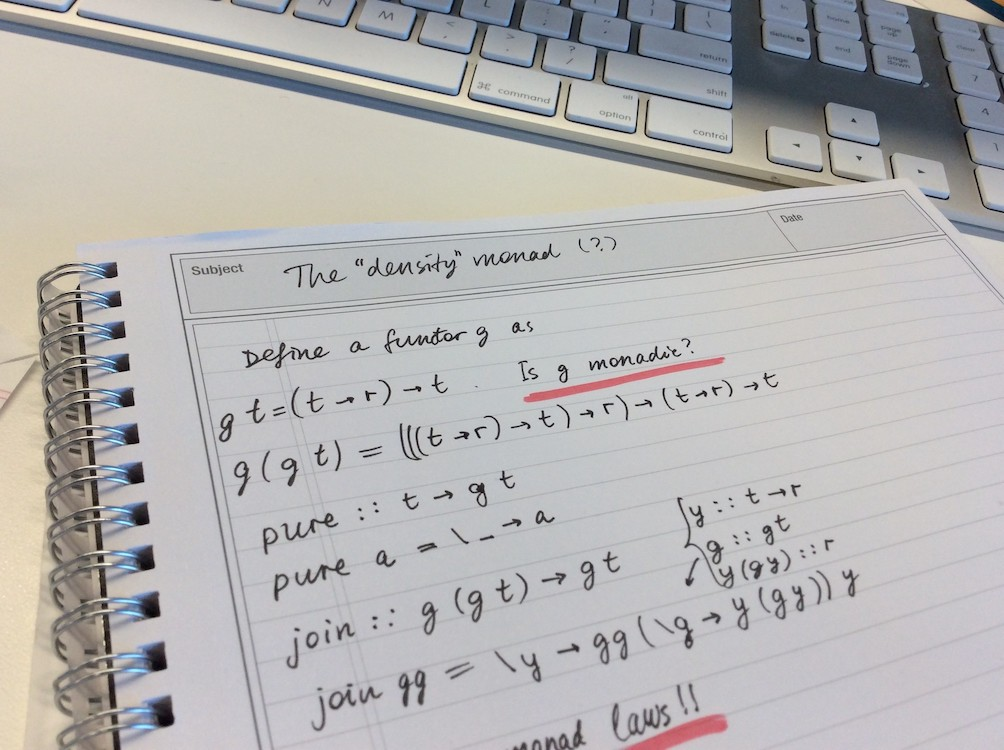
\includegraphics[width=0.6\linewidth]{ftt-example}}{\footnotesize\par}
\par\end{centering}
\caption{An imaginary programmer performs a derivation before writing Haskell
code.\label{fig:Example-calculation-in-type-theory}}

\end{figure}

A recent example of a development in applied functional type theory
is the \textsf{``}free applicative functor\textsf{''} construction. It was first described
in a 2014 paper.\footnote{\texttt{\href{https://arxiv.org/pdf/1403.0749.pdf}{https://arxiv.org/pdf/1403.0749.pdf}}}
A couple of years later, a combined free applicative / free monad
data type was designed and its implementation proposed in Scala\footnote{\texttt{\href{https://github.com/typelevel/cats/issues/983}{https://github.com/typelevel/cats/issues/983}}}
as well as in Haskell.\footnote{\texttt{\href{https://elvishjerricco.github.io/2016/04/08/applicative-effects-in-free-monads.html}{https://archive.is/kwD2a}}}
This technique allows programmers to implement declarative side-effect
computations where some parts are sequential but other parts are computed
in parallel, and to achieve the parallelism \emph{automatically} while
maintaining the composability of the resulting programs. The new technique
has advantages over monad transformers, which was a previously known
method of composing declarative side-effects. The combined \textsf{``}free
applicative / free monad\textsf{''} code was designed and implemented by true
software engineers. They first derived the type constructor that has
the necessary algebraic properties. Guided by the resulting type formula,
they wrote code that was guaranteed to work as intended.

Another example of using applied functional type theory is the  \textsf{``}\index{tagless final}tagless
final\textsf{''} encoding of effects, first described\footnote{\texttt{\href{http://okmij.org/ftp/tagless-final/index.html}{http://okmij.org/ftp/tagless-final/index.html}}}
in 2009. That technique (called \textsf{``}Church-encoded free monad\index{free monad}\textsf{''}
in the present book) has advantages over the ordinary free monad in
a number of cases \textemdash{} just as the free monad itself was
used to cure certain problems with monad transformers.\footnote{\texttt{\href{http://blog.ezyang.com/2013/09/if-youre-using-lift-youre-doing-it-wrong-probably/}{http://blog.ezyang.com/2013/09/if-youre-using-lift-youre-doing-it-wrong-probably/}}}
The new encoding is not tied to a specific programming language. Rather,
it is a language-agnostic construction that was originally described
in OCaml and later used in Haskell and Scala, but can be made to work
even in Java,\footnote{\texttt{\href{https://oleksandrmanzyuk.wordpress.com/2014/06/18/}{https://oleksandrmanzyuk.wordpress.com/2014/06/18/}}}
which is not an FP language.

This example shows that we may need several more years of work before
the practical aspects of using applied functional type theory are
sufficiently well understood by the FP community. The theory is in
active development, and its design patterns \textemdash{} as well
as the exact scope of the requisite theoretical material \textemdash{}
are still being figured out. If the 40-year gap hypothesis\footnote{\texttt{\href{https://www.linkedin.com/pulse/40-year-gap-what-has-academic-computer-science-ever-done-winitzki}{https://archive.is/kVYYt}}}
holds, we should expect applied functional type theory (perhaps under
a different name) to become mainstream by 2030. This book is a step
towards a clear designation of the scope of that theory.

\addsec{Does software need engineers, or are artisans sufficient? }

The demand for programmers is growing. \textsf{``}Software developer\textsf{''} was
\#1 best job\footnote{\texttt{\href{http://money.usnews.com/money/careers/articles/how-us-news-ranks-the-best-jobs}{http://money.usnews.com/money/careers/articles/how-us-news-ranks-the-best-jobs}}}
in the US in 2018. But is there a demand for engineers or just for
artisans?

We do not seem to be able to train enough software artisans.\footnote{\texttt{\href{http://archive.is/137b8}{http://archive.is/137b8}}}
So, it is probably impossible to train as many software engineers
in the true sense of the word. Modern computer science courses do
not actually train engineers in that sense. Instead, they train academic
researchers who will in most cases go on to work as software artisans
writing code.

Looking at the situation in construction business in the U.S.A., we
find that it employs about $40$ times more construction workers as
architects. We might conclude that perhaps one software engineer is
required per several dozen software artisans.

What is the price of \emph{not} having engineers, of replacing them
with artisans?

Software practitioners have long bemoaned the permanent state of \textsf{``}crisis\textsf{''}
in software development. Code \textsf{``}rots with time\textsf{''}, its complexity
grows \textsf{``}out of control\textsf{''}, and operating systems have been notorious
for a steady stream of new security flaws\footnote{\texttt{\href{http://archive.fo/HtQzw}{http://archive.fo/HtQzw}}}
despite many thousands of programmers and testers employed. It appears
that the growing complexity of software tends to overwhelm the capacity
of the human brain for correct \emph{artisanal} programming.

It is precisely in designing large and robust software systems that
we would benefit from true engineering. Artisans has been building
bridges and using chemical reactions by trial and error and via tradition,
long before mechanical or chemical engineering disciplines were developed
and founded upon rigorous theory. But once the theory became available,
engineers were able to design unimaginably more powerful and complicated
structures, devices, and processes. So, we may expect that trial,
error, and adherence to tradition is inadequate for some of the more
complex software development tasks in front of us. 

To build large and reliable software, such as new mobile or embedded
operating systems or distributed peer-to-peer trust architectures,
we will most likely need the qualitative increase in productivity
and reliability that can only come from replacing artisanal programming
by a true engineering discipline. Applied functional type theory and
functional programming are steps in that direction.

\addchap{Essay: Declarative programming as a silver bullet}

The main difficulty of software engineering is that programs tend
to grow in size and to become progressively less understandable. As
a result, bugs become hard or impossible to avoid as programmers need
to add new features. 

Initially, the paradigm of structural programming was supposed to
solve this problem. A famous paper, \textsf{``}No silver bullet\textsf{''},\footnote{\texttt{\href{https://en.wikipedia.org/wiki/No_Silver_Bullet}{https://en.wikipedia.org/wiki/No\_Silver\_Bullet}}}
rejected that view while at the same time doing little more than bemoaning
the mysterious difficulty of writing correct programs. Brooks blamed
it on the \textsf{``}inherent complexity\textsf{''} somehow present in all software
engineering because the domain problems being solved are complex.
Since then, people have claimed that object-oriented programming\footnote{\texttt{\href{http://www.drdobbs.com/there-is-a-silver-bullet/184407534}{http://www.drdobbs.com/there-is-a-silver-bullet/184407534}}}
or functional programming\footnote{\texttt{\href{http://archive.li/TE9iB}{http://archive.li/TE9iB}}}
are solutions to this difficulty; namely, that they will increase
productivity by order of magnitude while avoiding bugs. Many people
immediately stepped in to say that functional programming languages
\textemdash{} Lisp, Haskell, and such \textemdash{} are not a silver
bullet.\footnote{\texttt{\href{https://www.slideshare.net/nashjain/no-silver-bullets-in-functional-programming-by-brian-mckenna}{https://archive.is/pA1hz}}}

I think we actually do have a silver bullet, hiding in plain sight.
But rather than trying to argue from philosophical reasons, I would
like to look at practical results. What are historical examples where
a great increase in programmer productivity has been achieved by introducing
some new paradigm that proved sufficiently useful for most programming
languages to have adopted it later on?

After describing these past innovations, or \textsf{``}silver bullets\textsf{''},
we will be able to distill an underlying principle that drives the
productivity advantage. That principle is what I call declarative
programming. 

\addsec{The silver bullets we know and love}

Perhaps the first real silver bullet (after Alan Turing invented the
subroutine and the stack frame\footnote{\texttt{\href{https://people.cs.clemson.edu/~mark/subroutines.html}{https://people.cs.clemson.edu/$\sim$mark/subroutines.html}}})
came as one of the features of the Fortran language. That feature
of Fortran (that still survives in virtually all programming languages
today) is the math-like syntax for arithmetic expressions. With Fortran,
for the first time, the programmer could write a formula such as \lstinline!A = B * C - SQRT(D)!
and the computer would generate all the necessary machine codes for
computing that arithmetical expression. Before this innovation, programmers
would have to write out all the required elementary operations and
intermediate results in full, using machine instructions that corresponded
to the following sequence of actions:
\begin{lyxcode}
allocate~memory~1~(intended~for~A)

allocate~memory~2~(intended~for~B~{*}~C)

put~B~into~memory~2

multiply~memory~2~with~C~and~put~result~into~memory~2

allocate~memory~3~(intended~for~SQRT(D))

copy~register~0~into~memory~3~(to~save~it~for~later)

put~D~into~register~0

call~subroutine~SQRT~(expecting~result~again~in~register~0)

swap~register~0~and~memory~3~(now~restoring~old~register~0)

flip~sign~of~value~in~memory~3~(now~have~-SQRT(D)~in~memory~3)

add~memory~2~to~memory~3~and~put~result~into~memory~2

copy~memory~2~into~register~0

free~memory~2

free~memory~3

free~memory~1

return
\end{lyxcode}
Instead of this quite tedious and error-prone sequence of instructions,
Fortran programmers could simply write \lstinline!A = B * C - SQRT(D)!.
The order-of-magnitude productivity increase is obvious from this
example.

After Fortran, the LISP language enabled programmers to write recursive
computations on lists and trees quite easily. These kinds of computations
are important in two areas of computer science: compilers and strategy
games. Implementing a backtracking search without a direct access
to recursive data structures is a difficult and error-prone task.
Most programming languages today support recursive data structures
and recursive functions.

Another innovation was in the Prolog language. Prolog implemented
a backtracking search as a built-in feature that the programmer does
not even need to mention explicitly. A Prolog program only needs to
declare the logical relationships that define the search space. The
program may also specify shortcuts or speedups, to make the backtracking
search run more efficiently. Prolog, however, did not find a lot of
use outside the European artificial intelligence community of 1970\textendash 1980s.
Its best area of application (expert systems) has had its heyday and
is now a distant memory.

Nevertheless, the legacy of Prolog is alive and well in the form of
SQL, the relational database language. SQL simplified Prolog by removing
recursion, which made complicated search algorithms unnecessary, and
instead added various convenience features to support table-driven
accounting and reporting tasks. SQL is still a cornerstone of industrial
data processing today.

Object-oriented programming was initially intended, as in the SIMULA
language, for simulation of real-time interactions between systems.
It was thought that people would simply imagine how real-world objects
interact by sending each other requests or data, and transcribe that
picture into code. Later, it was argued that OOP is especially suitable
for developing a powerful graphical user interface, called OOUI.\footnote{\texttt{\href{https://en.wikipedia.org/wiki/Object-oriented_user_interface}{https://en.wikipedia.org/wiki/Object-oriented\_user\_interface}}}
Many programming languages today include some object-oriented features.

Functional programming languages started with Standard ML, which was
a language for programming a mathematical proof assistant. Languages
later developed in the spirit of Standard ML, such as OCaml and Haskell,
were mostly used for writing compilers and verified code. However,
basic features of Standard ML \textemdash{} immutable polynomial data
types, pattern-matching, higher-order functions, and parametric polymorphism
with a static type inference \textemdash{} have become standard, so
that many new languages (such as F\#, Scala, Swift, and Rust) include
them by design, while older languages (Java, C\#, Python) have retrofitted
some of these features. 

\addsec{What is \textquotedblleft declarative programming\textquotedblright}

I first encountered the concept of \textsf{``}declarative programming\textsf{''} when
I started studying Haskell and Prolog. Both languages are claimed
to be declarative, as opposed to imperative languages such as C++
or Java. It was confusing, however, that two languages that are so
different can be both deemed declarative. It was also clear that Prolog
would be quite awkward for, say, numerical calculations, while Haskell
would require a lot of hard-to-read, imperative code for tasks such
as downloading a file from a Web server. (The book \textsf{``}Real World Haskell\textsf{''}\footnote{\texttt{\href{https://amzn.com/dp/B0026OR2FY}{https://amzn.com/dp/B0026OR2FY}}}
shows some examples.\texttt{}\footnote{\texttt{\href{http://book.realworldhaskell.org/read/extended-example-web-client-programming.html}{http://book.realworldhaskell.org/read/extended-example-web-client-programming.html}}}\texttt{)}

I tried to understand what people mean by declarative programming.
The Wikipedia definition\footnote{\texttt{\href{https://en.wikipedia.org/wiki/Declarative_programming}{https://en.wikipedia.org/wiki/Declarative\_programming}}}
essentially says that declarative is \textsf{``}not imperative\textsf{''}, and yet
that definition is so vague that one could easily claim that Haskell
is imperative while Visual Basic is declarative. Essentially, \textsf{``}declarative\textsf{''}
is understood as a feature of a programming language as a whole, as
if any programming language could be argued to be either \textsf{``}declarative\textsf{''}
or not.

I was never satisfied with that definition and kept thinking about
this question until I found a better definition, which I will explain
now.

The common pattern among all the \textsf{``}silver bullet\textsf{''} paradigms is
that 1) they were supposed to make programs very concise and easily
readable when written for a specific and narrowly delineated problem
domain, 2) they came with a new programming language designed specifically
for that domain. Fortran was designed as a language for numerical
mathematics; Prolog as a language for rule-based expert systems; and
so on. One could plausibly argue that Fortran was as well adapted
to programming numerical expressions as Prolog to expert systems or
Haskell to compilers.

An important consequence is that the same languages were not suitable
for other problem domains! Prolog was not suitable for matrix multiplication,
nor Fortran for expert systems, nor Haskell for GUI programs.

Therefore, \textsf{``}declarativeness\textsf{''} is not  a property of a programming
language, but a \emph{relation} between a programming language and
a problem domain. A language can be declarative for one specific problem
domain but not for another.

The second important consequence is that a program in a \textsf{``}declarative\textsf{''}
language must be something that is clearly understandable to humans.
For example, the expression \lstinline!A = B * C - SQRT(D)! is unambiguous,
and its intent and effect are clear at first sight. This is because
the program closely resembles what a person would write on paper in
order to describe the required task. Similarly, Prolog programs look
like declarations of facts and logical relations between facts or
properties of some symbols. This is again very close to something
that a human would write informally on paper when describing a particular
task or problem.

Here is an example showing how Prolog is adapted to tasks involving
logical relations. Consider the following logic puzzle:
\begin{quotation}
All jumping creatures are green. All small jumping creatures are martians.
All green martians are intelligent. \noun{Ngtrks} is small and green.
\noun{Pgvdrk} is a jumping martian. Who is intelligent? \emph{(Inspired
by the short story \textsf{``}Invasion from Aldebaran\textsf{''}}\footnote{\texttt{\href{https://de.wikipedia.org/wiki/Invasion_vom_Aldebaran}{https://de.wikipedia.org/wiki/Invasion\_vom\_Aldebaran}}}\emph{
by S.~Lem.)}
\end{quotation}
The following is the complete code of the Prolog program that solves
this puzzle, together with an example execution command using SWI-Prolog:
\begin{lstlisting}[language=bash]
$ cat > martians.pl
small(ngtrks). green(ngtrks).
martian(pgvdrk). jumping(pgvdrk).
green(X) :- jumping(X).
martian(X) :- small(X), jumping(X).
intelligent(X) :- green(X), martian(X).

main :- intelligent(X), format('~w is intelligent.~n', X), halt.
^D
$ swipl -o martians -q -t main -c martians.pl
$ ./martians
pgvdrk is intelligent.
\end{lstlisting}
We could mechanically rewrite this code and replace Prolog predicates
such as \lstinline!green(X)! by phrases such as \textsf{``}\lstinline!X!
is green\textsf{''}, the Prolog operator \lstinline!:-! by the word \textsf{``}when\textsf{''},
and the comma (\lstinline!,!) by the word \textsf{``}and\textsf{''}. Then we would
find that the program code closely resembles the English-language
description of the puzzle. In this sense, Prolog programs can be viewed
as \textsf{``}executable specifications\textsf{''} for logic puzzles. 

However, writing a matrix multiplication program in Prolog would require
code that is far removed from any human-readable specification or
mathematical notation.\footnote{See, e.g., \texttt{\href{https://stackoverflow.com/questions/55687499}{https://stackoverflow.com/questions/55687499}}}
It is clear that Prolog is \emph{not} declarative for numerical calculations.

As an illustration of why Haskell is declarative for recursive data
structures, consider this excerpt from the book \textsf{``}Algorithms in C\textsf{''}\footnote{\texttt{\href{https://www.amazon.com/Algorithms-Parts-1-4-Fundamentals-Structures/dp/0201314525}{https://www.amazon.com/Algorithms-Parts-1-4-Fundamentals-Structures/dp/0201314525}}}
and its almost mechanical translation into Haskell code:
\begin{quotation}
\textbf{Definition 5.1} A binary tree is either an external node or
an internal node connected to a pair of binary trees, which are called
the left subtree and the right subtree of that node.
\end{quotation}
\begin{lstlisting}[language=Haskell]
data BTree a = BTNode a | BTVertex (BTree a) (BTree a)
\end{lstlisting}

\begin{quotation}
\textbf{Definition 5.6} The level of a node in a tree is one higher
than the level of its parent (with the root at level 0). The height
of a tree is the maximum of the levels of the tree\textsf{'}s nodes.
\end{quotation}
\begin{lstlisting}[language=Haskell]
heightOf :: BTree a -> Int
heightOf (BTNode _) = 0
heightOf (BTVertex left right) = 1 + max (heightOf left) (heightOf right)
\end{lstlisting}

These code snippets suggest that Haskell is declarative for the problem
domain of manipulating tree-like data structures via recursive algorithms.
Object-oriented implementations of these algorithms in C++ or Java
require significantly more code, and the code will not syntactically
resemble the specification. 

By looking at the \textsf{``}silver bullet\textsf{''} examples, we arrive at the following
definition of declarative programming:
\begin{quote}
\emph{A program is declarative if it syntactically resembles a human-written
specification of the required task, expressed in a commonly used specification
language. }
\end{quote}
It follows that the concept of \textsf{``}declarative programming\textsf{''} is actually
still narrower than a relation between a language and a problem domain.
Given the same programming language, a program for the same problem
domain can be written in different ways. Some of these equivalent
programs will be non-declarative if they do not closely resemble a
human-readable specification of the task.

A programming language is \textbf{declarative for a chosen problem
domain} if it allows us to write declarative programs for that domain.
Declarative programs are executable but still human-readable specifications,
written within the syntactic conventions of a specific programming
language.

\addsec{Specification languages}

A key question remains: what exactly is a \textsf{``}human-readable specification\textsf{''}?
Again, we need to look at known history to understand what specification
languages people have been using to communicate tasks in various problem
domains.

Mathematicians have spent millennia developing adequate notation for
the various tasks relating to numerical calculations and logical abstractions.
Writing the expression $A=B\cdot C-\sqrt{D}$ or the corresponding
code \lstinline!A = B * C - SQRT(D)! is as clear and unambiguous
as it gets when we want to talk about numerical formulas. We do not
know if another, \textsf{``}better\textsf{''} mathematical notation exists; but the
one we have today seems to work well enough.

Each domain where humans have developed sophisticated artifacts, such
as music, linguistics, technical drafting, and so on, has its own
specialized notation. These notations do not all have the same level
of formality or expressivity. For instance, the International Phonetic
Alphabet\footnote{\texttt{\href{https://en.wikipedia.org/wiki/International_Phonetic_Alphabet}{https://en.wikipedia.org/wiki/International\_Phonetic\_Alphabet}}}
denotes pronunciation rather precisely, but there seems to be no accepted
specification language that could denote unambiguously all the richness
of the expressive intonation people use when actually talking.

It is safe to say that the task of developing a \textsf{``}good\textsf{''} notation
\textemdash{} i.e., an unambiguous, expressive, and yet readable specification
language \textemdash{} for a given problem domain is a difficult task
that may take a long time for newer problem domains. The main reason
for the difficulty is that a successful specification language must
be convenient for human practitioners (whose detailed behavior, to
date, has evaded a formal description). A person reading a description
of a task in a good specification language must be able to understand
the task quickly and should have no further questions or ambiguities
to clarify.

It is precisely in areas where the specification language is well
understood (for example: mathematical formulas, formal grammars, relational
logic) that the development of a declarative programming language
produced an order of magnitude increase in productivity. In all those
cases, the programming language syntactically reproduces the specification
language and, in this sense, makes the specifications \textsf{``}executable\textsf{''}.
However, blind attempts to use the same language for other problem
domains did not bring any advantages. The widely expressed disappointments
with structural programming, natural-language programming, OOP, or
functional programming is probably due to the fact that people expected
a \textsf{``}declarativeness\textsf{''} in one domain to transfer to advantages in
all other problem domains. But this does not seem to be the case with
any of the attempts so far. Different problem domains are incompatible
and require quite different specification languages.

Without an accepted specification language, there is no hope of reaping
the full benefits of declarative programming. One domain where a specification
language seems to be currently lacking is the visual logic of GUI
applications. Several approaches \textemdash{} from business process
management formalisms to temporal logic \textemdash{} have been tried,
but so far no consensus emerged that any of those notations is truly
declarative, \textemdash{} that is, unambiguously expressive and at
the same time readily understandable to humans. When people design
GUIs, they communicate their designs to each other informally and
in multiple stages, gradually resolving the inevitable ambiguities.
(\textsf{``}And what if I now press this button in that window while the old
message box is still visible?\textsf{''}) As a result, GUI programming remains
a difficult and error-prone exercise. Established GUI environments
(X Window, MS Windows, macOS, iOS, Android) predominantly use the
object-oriented paradigm, which turned out to be not a silver bullet
for complex GUI design. Accordingly, programming a GUI application
in these environments is a messy and painful affair (I am speaking
from first-hand experience). Newer developments based on functional
reactive programming are more promising but yet to be proven declarative,
since no adequate specification language has emerged as yet in that
area. 

\addsec{How to use the silver bullet today: make your own DSL}

In the 1980s, 1990s, and 2000s, many companies (including IBM, Microsoft,
Sun, Apple, SAP, Bloomberg, and Workday) invented their own programming
languages adapted to their respective business domains. The idea was
that a specialized programming language would be necessary to serve
their specific business. I think their intuition was that not merely
that existing programming languages were not well adapted for business
applications, but also that the newly designed programming languages
would be made declarative for those domains. However, those companies
most likely did not have a precise definition of their specification
languages or problem domains before designing their new languages,
which thus did not necessarily achieve the goal of being declarative.

Suppose you know the specification language of your problem domain,
and you would like to create a language adapted to that domain, i.e.,
a domain-specific language (DSL). It takes a great deal of work to
create and support an entirely new programming language. The return
on the investment is relatively small.

A better approach is to implement your DSL as a library in an established
programming language (the \textsf{``}host\textsf{''} language). This produces a so-called
embedded DSL (EDSL). The EDSL does not need to be particularly complicated
or extensive. Its goal is to fit your problem domain so that you can
express specifications for your tasks syntactically, more or less
as you would tell them to a fellow human.

The immediate next question is to identify programming languages that
allow us to easily implement domain-specific languages. Several language
features seem to be required of a good \textsf{``}DSL-friendly\textsf{''} host language.
One is the ability to redefine the meaning of existing operations,
to fit the human-readable specification language. For example, we
might want to redefine (\textsf{``}overload\textsf{''}) the multiplication operator
(\lstinline!*!) so that \lstinline!m * n! would mean the matrix
multiplication when \lstinline!m! and \lstinline!n! are matrices.
C++, Python, Haskell, and Scala support operator overloading, but
Java and JavaScript do not.

Another useful feature would be the ability to make syntax shorter
and more easily understandable. For example, the \lstinline!scalatest!
library for Scala defines syntax that allows programmers to write
test conditions resembling English sentences, such as:
\begin{lstlisting}
a + b should be > 0
\end{lstlisting}
This code is more easily readable than an equivalent Java syntax:
\begin{lstlisting}
(a + b).should().be().greaterThan(0)
\end{lstlisting}

Another DSL-friendly feature is the ability to generate or transform
programs at compile time. For instance, a database DSL could read
the database schema at compile time and generate the data access layer
code, freeing the programmer from the tedious mechanical task of writing
and updating the code each time the schema is revised. If a host language
supports these features, a programmer can easily implement their own
little DSL adapted specifically to the problem domain at hand, without
modifying the host language\textsf{'}s compiler or creating an entirely new
programming language.

Finally, a DSL is hard to use if it is \textsf{``}brittle\textsf{''}, \textemdash{}
that is, permitting users to easily write correct-looking but buggy
programs. The key to assuring correctness is to be able to verify,
preferably at compile time (but in any case early in the development
cycle), that the user\textsf{'}s DSL program is consistent within the intended
meaning of the DSL. For instance, if the DSL allows us to multiply
matrices by writing \lstinline!m * n!, we should not be able to write
\lstinline!m * n! by mistake when \lstinline!n! is a telephone number
rather than a matrix, only to discover the error much later when the
code is running in production. The host language must maintain strict
control over the abstractions behind the DSL.

Because of the importance of DSL-friendly features, some programming
languages are more suitable to building DSLs than others. In particular,
Scala and Haskell have outstanding abilities to redefine syntax, prevent
user mistakes, perform compile-time code generation or transformation,
and hide complexity behind tightly controlled abstractions, \textemdash{}
all without modifying the existing compiler or tooling. For this reason,
it is much easier to create custom DSLs in Scala and Haskell than
in most other programming languages. 

\addsec{Conclusion}

Declarative programs are executable specifications. Thanks to the
development of modern programming languages such as Scala and Haskell,
the silver bullet is in our hands today. Just follow these easy steps
and you will slay the software werewolf!
\begin{enumerate}
\item Discover or develop a good specification language for your problem
domain. The specification language should be unambiguously expressive,
complete for the problem domain, pragmatically convenient, and yet
human-readable. It should be obvious at first reading that the specification
says exactly what we intend to do.
\item Learn Scala and/or Haskell. 
\item Implement the specification language syntactically as a DSL in a chosen
host language. Iterate on the language as necessary to support your
problem domain. 
\item If you have different problem domains in the same project, do not
mix different DSLs into one uber-language; this has proven to be counterproductive.
It is best to keep DSLs separate and independent.
\end{enumerate}

